\documentclass[Lau,binding=0.6cm]{sapthesis}

\usepackage{microtype}
\usepackage[english, italian]{babel}
\usepackage[utf8]{inputenx}

\usepackage{hyperref}
\hypersetup{pdftitle={Proprietà di sicurezza nel linguaggio Rust},pdfauthor={Edoardo De Matteis}}

\usepackage{listings, float, graphicx, lipsum, cleveref, parallel, verbatim, mathtools, ebproof, comment}
\usepackage{amssymb, pifont}
\usepackage[square, sort, comma, numbers]{natbib}
\usepackage[dvipsnames]{xcolor}
\usepackage[nottoc]{tocbibind}
\usepackage[most]{tcolorbox}
\usepackage[binary-units=true]{siunitx}
\usepackage[autostyle=true]{csquotes}

% theorem box
\newtcbtheorem[number within=chapter]{Definizione}{}{
    enhanced,
    sharp corners,
    attach boxed title to top left={
        xshift=-1mm,
        yshift=-5mm,
        yshifttext=-1mm
    },
    top=1.5em,
    colback=white,
    colframe=white!50!black, %rendere solo bianco
    fonttitle=\bfseries,
    boxed title style={
        sharp corners,
        size=small,
        colback=white!50!black,
        colframe=white!50!black,
    } 
}{def}


\newtheorem{theorem}{Theorem}[section]
\newtheorem{corollary}{Corollary}[theorem]
\newtheorem{lemma}[theorem]{}

\newenvironment{myDefinition}[2]{ \begin{Definizione}[adjusted title=#1]{}{#2}
    \textbf{Definizione \thetcbcounter.} }{\end{Definizione}}

\definecolor{codegreen}{rgb}{0,0.6,0}
\definecolor{codegray}{rgb}{0.5,0.5,0.5}
\definecolor{codepurple}{rgb}{0.58,0,0.82}
\definecolor{backcolour}{rgb}{0.95,0.95,0.92}

\lstdefinelanguage{Rust}{
  keywords={},
  otherkeywords={% Operators
    0x, 0o, 0b,
    i8, i16, i32, i64, i32, i128, isize, 
    u8, i16, u32, u64, u32, u128, usize, 
    f8, f16, f32, f64, f32, f128, fsize
  },
  keywords = [2]{fn, if, in, for, let, match, struct, unsafe, while},
  keywords = [3]{as, const, move, mut},
  keywordstyle=\color{codepurple},
  keywordstyle=[2]\color{MidnightBlue},
  keywordstyle=[3]\color{Rhodamine},
  comment=[l]{//},
  morecomment=[s]{/*}{*/},
  commentstyle=\color{codegreen}\ttfamily,
  stringstyle=\color{orange}\ttfamily,
  morestring=[b]"
  }

\lstdefinestyle{mycode}{
    backgroundcolor=\color{backcolour},   
    commentstyle=\color{codegreen},
    keywordstyle=\color{MidnightBlue},
    numberstyle=\tiny\color{codegray},
    stringstyle=\color{orange},
    basicstyle=\ttfamily\footnotesize,
    breakatwhitespace=false,         
    breaklines=true,                 
    captionpos=b,                    
    keepspaces=true,                 
    numbers=left,                    
    numbersep=5pt,                  
    showspaces=false,                
    showstringspaces=false,
    showtabs=false,                  
    tabsize=2
}

\lstset{style=mycode}

% command for inline code
\newcommand{\textcode}[1]{\colorbox{backcolour}{\texttt{#1}}}

% checkmark and x mark
\newcommand{\cmark}{\ding{51}}
\newcommand{\xmark}{\ding{55}}

% Commands for the titlepage
\title{Proprietà di sicurezza nel linguaggio Rust}
\author{Edoardo De Matteis}
\IDnumber{1746561}
\course{Informatica}
\courseorganizer{Facoltà di Ingegneria dell'informazione, informatica e statistica}
\AcademicYear{2019/2020}
\copyyear{2020}
\advisor{Pietro Cenciarelli}
%\advisor{Dr. Nome Cognome}
%\coadvisor{Dr. Nome Cognome}
\authoremail{edoardodematteis@icloud.com}

%\examdate{16 April 2013}
%\examiner{Prof. Nome Cognome}
%\examiner{Prof. Nome Cognome}
%\examiner{Dr. Nome Cognome}
\versiondate{\today}

\begin{document}

\frontmatter

\maketitle

%\dedication{Dedicato a\\ Donald Knuth}

%\begin{abstract}
%\end{abstract}

%\begin{acknowledgments}
%\end{acknowledgments}

\tableofcontents

% Do not use the starred version of the chapter command!

\mainmatter

\chapter{Introduzione}

Il linguaggio di programmazione C è stato sviluppato nel 1978 e ad oggi è ancora uno dei più popolari ~\cite{tiobe:index} ~\cite{pypl:index}, ciò è dovuto al fatto che circa il 98\% ~\cite{real_men_program_in_c} dei sistemi informatici sul mercato siano sistemi integrati che richiedono un basso overhead e C risponde a questa esigenza tramite una gestione manuale della memoria, l'esecuzione dei programmi consuma quindi meno risorse ma si richiede un maggiore impegno da parte del programmatore, è infatti suo compito allocare memoria adeguatamente e successivamente liberarla. 
Rimettendo totalmente al programmatore la gestione della memoria C permette di scrivere programmi non sicuri, esistono linguaggi come Java considerati sicuri che gestiscono automaticamente la memoria tramite \textbf{garbage collection} (definizione \ref{def:garbage_collection}) al prezzo di un maggiore overhead, sono quindi poco adatti alla scrittura di codice per embedded systems.

\begin{myDefinition}{Garbage collection}{garbage_collection}
    È una delle tecniche di gestione automatica della memoria più usate nei linguaggi di programmazione: tramite un modulo noto come \textbf{garbage collector} si tiene traccia di ogni allocazione e le zone di memoria non più necessarie vengono periodicamente liberate, rendendole nuovamente disponibili. 
    La garbage collection ha il vantaggio di esonerare il programmatore dal dover gestire la memoria per potersi concentrare sulla logica del programma e la sua leggibilità, si evitano inoltre vulnerabilità quali double free o dangling pointer (rispettivamente sezioni \ref{sec:double_free} e \ref{sec:dangling_reference}). 
    Con la garbage collection l'esecuzione dei programmi è più lenta data la presenza del garbage collector.
\end{myDefinition}

Nel breve futuro ci si aspetta sempre un numero crescente di oggetti d'uso comune connessi tra loro (i.e. internet of things) e si sente la necessità di metodi sicuri per programmare sistemi integrati. 
Nella ricerca di un linguaggio sicuro con gestione esplicita della memoria Rust sembra essere il miglior candidato grazie ai \textbf{lifetime}, questi descrivono lo scope nel quale una variabile è valida e sono fondamentali per il corretto funzionamento dei meccanismi di \textbf{ownership} e \textbf{borrowing}, dal momento che la loro verifica avviene a tempo di compilazione l'esecuzione dei programmi ne guadagna in velocità. 
I due obiettivi di Rust sono infatti sicurezza e velocità d'esecuzione dei suoi programmi: la prima è garantita dall'ownership che impedisce il manifestarsi di \textbf{side effect} (definizione \ref{def:side_effect}), la seconda sia tramite il maggior numero possibile di controlli statici che tramite borrowing il quale simula una call by reference - in Rust come in C c'è solo call by value. 

\begin{myDefinition}{Side effect}{side_effect}
    Un programma presenta side effect quando contiene almeno un'operazione che modifica lo stato di una o più variabili non presenti nel suo ambiente locale.
    I side effect non sono necessariamente negativi, variabili globali e processi concorrenti acquistano la loro forza proprio da questi effetti collaterali.
\end{myDefinition}

\chapter{Rust}

\section{Sistemi di tipi substrutturali}

I sistemi di tipi \textbf{substrutturali} sono una famiglia di sistemi di tipi (capitolo \ref{chap:type_safety}) dove almeno una delle seguenti proprietà - dette \textbf{strutturali} - non è presente o lo è sotto determinate condizioni, allo stesso modo si parlerà anche di logiche substrutturali.

\begin{lemma}[Exchange] \label{lemma:exchange}
    L'ordine degli elementi all'interno di un'ipotesi o conclusione è irrilevante.
\end{lemma}

\begin{lemma}[Weakening] \label{lemma:weakening}
    L'ipotesi e la conclusione possono essere estese con affermazioni non rilevanti senza alcuna ripercussione. 
\end{lemma}

\begin{lemma}[Contraction] \label{lemma:contraction}
    In ipotesi o conclusione è possibile sostituire due membri con un terzo, a patto che entrambi siano nella stessa espressione e che siano effettivamente unificabili.
\end{lemma}

Un'interpretazione delle logiche e dei sistemi substrutturali permette di ragionare in termini di consumo di risorse, vincolandone l'accesso e tenendo traccia dei cambiamenti di stato della memoria evitando stati non validi. 

In un esempio del 1987 Tony Hoare suppone di rappresentare in logica del primo ordine il fatto di avere una caramella con il predicato \textit{candy} e con  \textit{\$1} il possesso di un dollaro, per esprimere l'atto di compravendita di una caramella possiamo scrivere $ \textit{\$1} \rightarrow \textit{candy} $.

\begin{equation*}
  \begin{prooftree}
    \hypo{\textit{\$1} \rightarrow \textit{candy}}
    \hypo{\textit{\$1}}
    \infer2[modus ponens]{\textit{candy}}
  \end{prooftree}
\end{equation*}

Se ne deduce $ \textit{\$1} \land \textit{candy} $ e si ha una caramella senza aver pagato, si può evitare questo problema con modellazioni differenti della base di conoscenza ma si incorre nel \textit{frame problem} \footnote{In intelligenza artificiale è il problema di dover rappresentare una conoscenza in logica senza ricorrere a numerosi assiomi i quali indicano solo che l'ambiente non cambia arbitrariamente.}. 

\begin{table}[h!t]
    \centering
    \caption{Sistemi di tipi substrutturali.}
    \label{tab:substructural_type_systems}
    \begin{tabular}{c|ccc}
        & \textbf{Exchange} & \textbf{Weakening} & \textbf{Contraction} \\
        \hline
        \textbf{Rilevante} & \cmark & \xmark & \cmark\\
        \textbf{Affine} & \cmark & \cmark & \xmark\\
        \textbf{Lineare} & \cmark & \xmark & \xmark\\
        %\textbf{Ordinato} & \xmark & \xmark & \xmark\\
    \end{tabular}
\end{table}

Nella tabella \ref{tab:substructural_type_systems} è presentata una corrispondenza tra alcuni sistemi substrutturali e le regole in esso valide: in un sistema di tipi rilevante dal momento che non vale la regola di weakening non è possibile avere risorse superflue e ognuna dovrà essere usata almeno una volta. 
La definizione del verbo "usare" è ambigua e dipende dall'implementazione del linguaggio, si può definire un insieme di azioni e quando si afferma di usare una risorsa ci si riferisce all'esecuzione su questa di una delle azioni possibili, in Rust ad esempio sono specificate dalle regole di ownership.

In un sistema affine non è valida la contraction, questo implica che due usi differenti della stessa risorsa non possano essere unificati in uno solo e in un programma si può tradurre con l'impossibilità di liberare due volte la stessa zona di memoria (\ref{sec:double_free}); un sistema o una logica lineare ~\cite{girard:linear_logic} è sintesi di uno rilevante e un affine quindi vale solo exchange, ogni risorsa deve essere usata esattamente una volta.
Nella sintassi di una logica lineare sono presenti dei qualificatori che marcano una variabile come lineare indicando che debba essere usata una volta.

In un sistema lineare per garantire la non riusabilità di una variabile vengono imposte due invarianti ~\cite{walker:linear_logic}:

\begin{enumerate}
    \item Le variabili lineari sono usate esattamente una volta per ogni cammino nel diagramma di flusso.
    \item Espressioni meno restrittive non possono contenere espressioni più restrittive. 
\end{enumerate}

Il perché la prima invariante sia fondamentale è chiaro, dopotutto è proprio il nostro obiettivo; per la seconda supponiamo di avere un oggetto \texttt{X} non lineare e un suo attributo \texttt{X.y} lineare, sarebbe possibile sfruttare \texttt{X} per usare più volte \texttt{X.y}, si avrebbe in questo modo una violazione della linearità. 

\section{Linearità in Rust}

Rust presenta un sistema dei tipi lineare e tutte le variabili sono marcate come lineari tranne quelle di tipo primitivo, le invarianti sulla linearità vengono rispettate tramite ownership e borrowing.

L'ownership rappresenta il possesso di un right value da parte di un left value (definizione \ref{def:left_right_value}), in Rust gli oggetti di tipo composto sono lineari e solo a questi si applica ownership, al momento dell'inizializzazione di un oggetto la sua variabile, se presente, è l'unico owner e un assegnamento ad una seconda variabile fa passare il possesso dalla prima alla seconda: in qualsiasi momento quindi può esserci solo un possessore per ogni oggetto. 
Un owner viene invalidato con la sua distruzione quando esce dal suo scope, bisogna porre particolare attenzione in questo caso dato che le chiamate di funzioni possono invalidare una variabile passata come argomento: il possesso passa alla nuova variabile nel corpo della funzione e una volta terminato il suo scope non sarà più possibile accedere all'oggetto con la variabile vecchia, in quanto si può avere massimo un owner per volta, né con la nuova poiché ormai si è fuori dal suo scope (listato \ref{lst:ownership}). 

\lstinputlisting[language=Rust,caption={Ownership}, label={lst:ownership}]{../code/Ownership/own.rs}

\begin{myDefinition}{Left e Right value}{left_right_value}
    Dato un assegnamento un left value punta ad un'area di memoria contenente un right value, il nome è dovuto alla posizione dei due valori rispetto all'operatore di assegnamento: in \textcode{x = y} il left value è \textcode{x} e il right \textcode{y}.
\end{myDefinition}

L'ownership è fondamentale per garantire una gestione automatica e sicura della memoria senza garbage collector ma non è sempre desiderabile prendere possesso di un oggetto, in questi casi si ricorre al borrowing.

Tramite il borrowing si possono creare molteplici  riferimenti ~\cite[4.2]{rust:language} ad un dato purché in sola lettura, con il modificatore \textcode{mut} è possibile rendere il riferimento modificabile a patto che in qualsiasi momento per qualsiasi variabile ve ne sia al più uno. 
Un modulo chiamato \textbf{borrow checker} garantisce a tempo di compilazione che finché esistono dei riferimenti ad un oggetto non sia possibile distruggere l'oggetto in questione. 

\lstinputlisting[language=Rust,caption={Borrowing}, label={lst:borrowing}]{../code/Borrowing/borr.rs}

Un lifetime è un costrutto usato dal borrow checker per garantire che ogni riferimento sia valido, il lifetime di una variabile inizia quando questa viene creata e termina quando viene distrutta; il compilatore quando possibile inferisce i lifetime, in caso contrario è necessario gestirli manualmente.

I lifetime sono delle regioni di codice nella quale ogni riferimento deve essere valido ~\cite[3.3]{rust:rustonomicon} ma è facile confondere scope e lifetime, negli esempi più semplici coincidono ma i secondi esprimono relazioni tra scope: un lifetime può essere associato a più scope e uno scope può avere associati più lifetime. 

Per quanto concerne i lifetime in Rust valgono tre regole assiomatiche ~\cite{mechpen:misundestand}:

\begin{lemma}[Association] \label{lemma:association}
    Dato un riferimento il suo scope è sottoinsieme del suo lifetime.
    \begin{equation*}
        \textnormal{\textcode{x:\&'a T}} \longrightarrow  scope(x) \subseteq \ 'a
    \end{equation*}
\end{lemma}

\begin{lemma}[Reference] \label{lemma:reference}
    Un lifetime associato ad un riferimento è sottoinsieme dello scope dell'oggetto cui fa riferimento. 
    \begin{equation*}
        \textnormal{\textcode{x:\&'a T = \&y}} \longrightarrow \ 'a \subseteq scope(y)
    \end{equation*}
\end{lemma}

\begin{lemma}[Assignment] \label{lemma:assignment}
    Un lifetime associato ad un riferimento è sottoinsieme del lifetime dell'oggetto cui fa riferimento.
    \begin{equation*}
        \textnormal{\textcode{x:\&'a S = y: \&'b T}} \longrightarrow \ 'a \subseteq \ 'b
    \end{equation*}
\end{lemma}

e ne deriva una quarta regola:

\begin{lemma}[Struct reference] \label{lemma:struct_reference}
    Data una struct \textnormal{\textcode{struct S<'a>\{x:\&'a T\}}} il lifetime associato ad un riferimento di una struct è sottoinsieme del lifetime del membro della struct\footnote{Nel caso in cui dovessero esserci più elementi con lifetime differenti si può considerare il maggiore.}.
    \begin{equation*}
        \textnormal{\textcode{s:\&'b S<'a>}} \longrightarrow \ 'b \subseteq \ 'a
    \end{equation*}
    Dimostrazione: \textnormal{Per \textnormal{\textcode{s:\&'b S<'a>}} esiste un \textcode{y:S<'a>} tale che \textcode{s:\&'b S = \&y} e applicando \ref{lemma:reference} e \ref{lemma:association} si ha} $ 'b \subseteq scope(y) = scope(y.x) \subseteq \ 'a  $.
\end{lemma}

% double reference non la scrivo perché non so neanche se sia legale in Rust

e si hanno delle regole speciali:
\begin{itemize}
    \item Il lifetime speciale \textcode{'static} rappresenta lo scope globale, ogni lifetime è suo sottoinsieme $ 'a \subseteq \ 'static $
    \item La \textbf{coercion} permette di forzare un lifetime più lungo in uno più breve $ \textnormal{\textcode{'a:'b}} \leftrightarrow 'a \subseteq \ 'b $
\end{itemize}

Si parla di \textbf{outliving} quando per una variabile è possibile mantenere il riferimento di un oggetto distrutto. 
Nelle righe 2 e 5 del listato \ref{lst:lifetime_1} si possono applicare rispettivamente le regole \ref{lemma:association} e \ref{lemma:reference} per dedurre $ scope(x) \subseteq \ 'a $ e $ 'a \subseteq scope(y) $, è noto $ scope(y) \subset scope(x) $ quindi il borrow checker interviene.

\lstinputlisting[language=Rust]{../code/Lifetime/life_1.rs}
\lstinputlisting[caption={Outliving e borrow checker.}, label={lst:lifetime_1}, numbers=none]{../code/Lifetime/output/life_1.txt}

Si può ottenere outliving cambiando il tipo di \textcode{y} da \textcode{i32} a \textcode{\&i32} (listato \ref{lst:lifetime_1_1}), così facendo non è possibile applicare \ref{lemma:reference} e vale $ scope(y) \subset scope(x) \subset \ 'a $. 
Un comportamento del genere è inaspettato ma è stato reso possibile per semplificare la definizione di variabili costanti statiche di tipo primitivo ~\cite{git:outliving_static}, i riferimenti ai letterali vengono allocati in memoria di default staticamente e non automaticamente (capitolo \ref{chap:memory_safety}) creando un riferimento con lifetime \textcode{'static}, dunque ogni riferimento ad un dato di tipo primitivo è valido per la durata di tutto il programma.

\lstinputlisting[language=Rust]{../code/Lifetime/life_1_1.rs}
\lstinputlisting[caption={Outliving.}, label={lst:lifetime_1_1}, numbers=none]{../code/Lifetime/output/life_1_1.txt}

In Rust i tipi composti sono costituiti da una struct, nel listato \ref{lst:lifetime_1_2} si può vedere la situazione precedente ma con un tipo non primitivo: nella riga 2 si ha $ scope(x) \subseteq \ 'a $ per \ref{lemma:association} e $ 'a \subseteq scope(y) \subseteq \ 'b$ per \ref{lemma:struct_reference}, è noto $ scope(y) \subset scope(x) $ ed essendoci una contraddizione il borrow checker interviene.  

\lstinputlisting[language=Rust]{../code/Lifetime/life_1_2.rs}
\lstinputlisting[caption={Outliving con tipi composti.}, label={lst:lifetime_1_2}, numbers=none]{../code/Lifetime/output/life_1_2.txt}

Nell'errore in output si parla di \textbf{temporary}: è una variabile anonima inizializzata con il risultato di un'espressione, verrà usata per le successive valutazioni e perderà validità solo al termine del suo scope come qualsiasi variabile. 
A \textcode{Box::new(13)} corrisponde una temporary e quando si tenta di leggerne il valore fuori dal suo scope il compilatore segnala l'errore. 

Negli esempi precedenti i lifetime sono sempre stati inferiti ma nel listato \ref{lst:lifetime_longest} sono esplicitati, si ha:
\begin{gather*}
    scope(rs1) \subseteq \ 'a \subseteq scope(s1) \\
    scope(rs2) \subseteq \ 'a \subseteq scope(s2) \\
    scope(result) \subseteq \ 'a \\
\end{gather*}

che è soddisfatto con $ 'a = scope(result) $.

\lstinputlisting[language=Rust]{../code/Lifetime/life_longest.rs}
\lstinputlisting[caption={Lifetime espliciti.}, label={lst:lifetime_longest}, numbers=none]{../code/Lifetime/output/life_longest.txt}

Quando a seguito di un assegnamento la variabile memorizza un riferimento ad un oggetto si parla di \textbf{shallow copy}, se invece si memorizza il dato per intero si ha una una \textbf{deep copy}. 
In Rust per i dati di tipo primitivo si eseguono sempre deep copy mentre per gli oggetti composti si eseguono di default shallow copy, è comunque possibile copiare l'oggetto nella sua interezza tramite il \textbf{trait} (simile a quello che in Java è un'interfaccia) \textcode{Clone}; questo avviene poiché di un dato di tipo primitivo la dimensione è nota a tempo di compilazione ma non si può dire lo stesso degli oggetti composti. Nel listato \ref{lst:ownership_primitive} \textcode{x} e \textcode{y} puntano a due locazioni differenti.

\lstinputlisting[language=Rust, caption={Ownership con tipi primitivi.}, label={lst:ownership_primitive}]{../code/Ownership/own_prim.rs}

Se con ownership e borrowing l'esecuzione di un programma è molto più rapida e sicura il linguaggio è più verboso e richiede maggior impegno cognitivo da parte del programmatore. 


\chapter{Security policy} \label{chap:security_policy}

Risulta molto difficile parlare di sicurezza in generale dato che non ne esiste una definizione assoluta ma è un concetto relativo che varia in base a cosa ci interessa proteggere e garantire. 
La sicurezza di un'organizzazione - che essa sia una multinazionale o un singolo individuo - è definita da una \textbf{security policy}  ovvero un documento contenente regole, principi e pratiche che determinano come garantire che il sistema si trovi in uno stato sicuro ~\cite{milner:type_polymorphism}. 

\begin{myDefinition}{Security policy}{security_policy}
    In una politica di sicurezza si definiscono quali azioni i \textbf{principal} possono eseguire sugli oggetti. Un principal è un'entità qualsiasi che interagisce con il sistema e deve rispettare la politica di sicurezza, nel caso specifico dei linguaggi di programmazione saranno entità software.
\end{myDefinition}

Nello sviluppo di linguaggi di programmazione sicuri si è guidati da due principi ~\cite{nino:security_programming_language}:
\begin{itemize}
    \item \textbf{Trusted computing base (TCB)}. Un sistema presenta componenti critici per il rispetto della policy, questi formano il TCB ed è fondamentale non presenti vulnerabilità dato che metterebbero a repentaglio la sicurezza del sistema stesso, il TCB deve essere semplice e limitato così da poterne verificare facilmente la correttezza ed evitare fallimenti. 
    \item \textbf{Principle of Least Privilege (POLP)}. Durante l'esecuzione ogni entità deve avere il numero minore possibile di permessi necessari per eseguire il suo compito. 
\end{itemize} 
È possibile scomporre i requisiti di sicurezza fondamentali durante lo sviluppo in \textbf{access control} e \textbf{information flow}, il primo limita chi o cosa possa accedere a quali risorse e il secondo definisce quali operazioni siano corrette o meno in seguito ad un accesso conforme all'accesso control, di norma il sistema operativo stesso implementa questi controlli via software o hardware e programmi che sono legali in C potrebbero comunque essere interrotti. 
In Rust la sicurezza è garantita da regole semplici e verificabili e si rispetta il POLP, i controlli sono eseguiti a tempo di compilazione e anche quando un programma viene interrotto a runtime non viene scomodato il sistema operativo (vedere ad esempio il codice nel listato \ref{lst:integeroverflowrs}).

Questa necessità di implementare la sicurezza nel linguaggio stesso e non rimetterla più nelle mani del sistema operativo è nata dall'avvento di internet e la sempre più grande condivisione di codice potenzialmente pericoloso.

Per dimostrare delle proprietà di un linguaggio serve una definizione formale della sua \textbf{semantica} ovvero l'insieme delle regole che definiscono il significato di un linguaggio e dei suoi programmi.
A tal proposito Rust non ha una semantica formale definita (figura \ref{fig:warning}) e la sua definizione di sicurezza è poco chiara, un programma è sicuro se rispetta \textbf{memory safety} (capitolo \ref{chap:memory_safety}) e \textbf{semantica statica} (capitolo \ref{chap:type_safety}) ~\cite[14]{rust:reference} ma la documentazione presenta delle definizioni poco chiare se non addirittura contraddittorie: 

\vspace{5mm}

\begin{Parallel}{0.48\textwidth}{0.48\textwidth}
    \selectlanguage{english}
    \ParallelLText{
        "Rust code is incorrect if it exhibits any of the behaviors in the following list. This includes code within \textcode{unsafe} blocks and \textcode{unsafe} functions. \textcode{unsafe} only means that avoiding undefined behavior is on the programmer; it does not change anything about the fact that Rust programs must never cause undefined behavior." ~\cite[14.3]{rust:reference}
    }
    
    \selectlanguage{italian}
    \ParallelRText{
        "Del codice in Rust non è corretto se presenta almeno uno dei comportamenti in lista. Questo vale anche per codice in blocchi \texttt{unsafe} e funzioni \textcode{unsafe}. \texttt{unsafe} significa solo che evitare undefined behaviour è compito del programmatore; non cambia alcuna garanzia sul fatto che i programmi in Rust non debbano mai causare undefined behaviour." 
    }
    \ParallelPar
\end{Parallel}

\vspace{5mm}

L'uso del termine "unsafe" è causa di confusione dal momento che \colorbox{backcolour}{\texttt{unsafe}} è un costrutto sintattico che consente la scrittura di codice che può causare \textbf{undefined behavior}, per questo si dice che Rust è composto da due "sottolinguaggi": \textit{unsafe Rust} e \textit{safe Rust} in base alla presenza o meno di un blocco \colorbox{backcolour}{\texttt{unsafe}} nel codice, questo costrutto è desiderabile perché permette sia di poter comunicare con librerie in \textit{C} che di avere un accesso più esplicito alla memoria ~\cite[1.2]{rust:rustonomicon}; piuttosto che una definizione formale di undefined behavior si ha una lista in continuo aggiornamento ~\cite[14.3]{rust:reference}, è importante notare che comunque safe Rust presenta del codice in blocchi \textcode{unsafe} scritto dagli sviluppatori.

Nella citazione riportata sono presenti fonti di confusione: nella stessa frase viene detto prima che in un blocco \textcode{unsafe} sia compito del programmatore evitare undefined behavior e subito dopo viene affermato come le garanzie sulla safety siano le stesse di safe Rust, quindi anche l'assenza di undefined behavior. 
Volendo comunque considerare solo l'ultima affermazione, l'esecuzione in un blocco \textcode{unsafe} di uno degli esempi in lista non dovrebbe causare undefined behavior; nel listato \ref{lst:unsafe_raw} si ha un \textbf{raw pointer dereferencing} (presente in lista come dimostrato in figura \ref{fig:warning}): è possibile leggere il valore memorizzato in una locazione di memoria tramite il suo indirizzo come in C.

È ragionevole che questo sia possibile solo in unsafe Rust ma mette in luce come la documentazione sia poco chiara. 

\lstinputlisting[language=Rust]{../code/Unsafe/raw.rs}
\lstinputlisting[caption={Raw pointer dereferencing in un blocco \texttt{unsafe}}, label={lst:unsafe_raw}, numbers=none]{../code/Unsafe/output/rawrs.txt}

\begin{figure}[h!t]
    \centering
    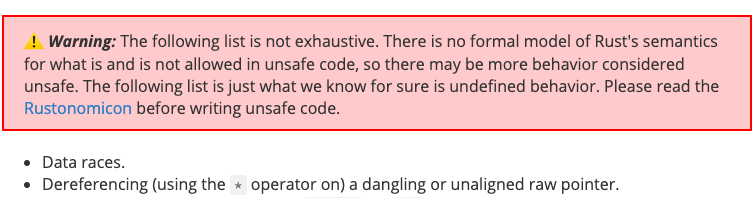
\includegraphics[scale=0.52]{images/warning_undefined_behavior.png}
    \caption{Il raw pointer dereferencing è considerato undefined behavior}
    \label{fig:warning}
\end{figure}


\chapter{Memory Safety} \label{chap:memory_safety}

Durante l'esecuzione di un programma ogni oggetto ha associato un insieme finito di locazioni di memoria cui accedere noto come \textbf{address space}, se in un programma nessun oggetto accede mai ad indirizzi fuori dal proprio address space allora è \textbf{memory safe} e un linguaggio che garantisce la memory safety dei suoi programmi è detto a sua volta memory safe.

L'address space può essere definito a tempo di compilazione o esecuzione dipendentemente dal tipo di allocazione, in C e Rust ne consideriamo tre tipi:

\begin{itemize}
    \item \textbf{Allocazione statica}. Il compilatore memorizza solo ed esclusivamente le variabili globali ovvero quelle il cui scope corrisponde a tutto il file, si possono definire tramite un modificatore (in C è \textcode{static}, da cui il nome) o definendole fuori da ogni funzione.  
    \item \textbf{Allocazione automatica}. Si usa per variabili locali e di tipo primitivo. Una variabile è locale quando dichiarata all'interno di una funzione (quindi valida solo in un determinato scope), dal momento che l'ordine di esecuzione non è noto a tempo di compilazione l'allocazione avviene a tempo di esecuzione e si utilizza una struttura dati nota come \textbf{stack} o \textbf{call stack}. 
    Spesso il nome call stack viene utilizzato per le sole chiamate di funzione. 
    \item \textbf{Allocazione dinamica}. L'allocazione dinamica in C è esplicita tramite funzioni come \textcode{malloc} e permette di allocare memoria ad un oggetto durante l'esecuzione, si rivela particolarmente utile con oggetti che non hanno dimensione fissa. 
    In safe Rust non si hanno funzioni del genere per questioni di sicurezza ma si ha il tipo \textcode{Box}, si usa una struttura dati chiamata \textbf{heap} che ha la particolarità di crescere verso l'alto, contrariamente allo stack che cresce verso il basso, e può essere problematico in caso di overflow (sezione \ref{sec:buffer_overflow}). 
    Un tipo composto è definito dall'unione di tipi primitivi e non è banale prevedere la dimensione di un oggetto composto quindi vengono allocati sull'heap. 
    Un oggetto di tipo primitivo viene salvato sullo stack. 
\end{itemize}

Questo approccio è stato reso popolare dal C ed è oggi adottato da numerosi linguaggi, sempre in C esiste un ulteriore tipo di allocazione della memoria noto come \textbf{register allocation} che permette di scrivere direttamente su un blocco del processore, non è presente in Rust.

\section{Buffer Overflow} \label{sec:buffer_overflow}
Un \textbf{buffer} è una qualsiasi zona contigua di memoria contenente istanze dello stesso dato e ne definisce i limiti, se durante l'esecuzione si riescono a superare si parla di \textbf{buffer overflow} ed è possibile leggere o scrivere oltre il proprio address space. 
Un esempio di buffer overflow in C è nel listato \ref{lst:stackoverflowc} ~\cite[7.5]{stallings:os}: dato che gli array sono posizionati uno dopo l'altro (in ordine LIFO essendo dati allocati su uno stack) si riesce a leggere e scrivere su \textcode{str1} eludendo anche il controllo di uguaglianza, nel terzo caso questo controllo viene superato perché si confrontano solo i primi 8 caratteri.
In Rust questo non è possibile, si veda nel listato \ref{lst:bufofrs} come il linguaggio esegua dei controlli sulle dimensioni degli array, esattamente ciò che la funzione \textcode{gets} non fa. 

\lstinputlisting[language=C]{../code/BufferOverflow/StackOverflow/StackAttack/stackattack.c}
\lstinputlisting[numbers=none]{../code/BufferOverflow/StackOverflow/StackAttack/output/stackattack_1_c.txt}
\lstinputlisting[numbers=none]{../code/BufferOverflow/StackOverflow/StackAttack/output/stackattack_2_c.txt}
\lstinputlisting[caption={Buffer overflow in C}, label={lst:stackoverflowc}, numbers=none]{../code/BufferOverflow/StackOverflow/StackAttack/output/stackattack_3_c.txt}

\lstinputlisting[language=Rust]{../code/BufferOverflow/bufof.rs}
\lstinputlisting[caption=Buffer overflow in Rust, label={lst:bufofrs}, numbers=none]{../code/BufferOverflow/output/bufof_rs.txt}

La pericolosità del buffer overflow è dovuta alla possibilità di attuare una \textbf{code injection} ovvero eseguire codice arbitrario, nel listato \ref{lst:injection} se ne ha un esempio molto semplice, per la stringa in input non si ha alcun tipo di bound check ed è possibile scrivere un comando che verrà eseguito da \textcode{system()} con gli stessi permessi con cui si esegue il file. 

\lstinputlisting[language=C]{../code/Injection/inj.c}
\lstinputlisting[caption={Code injection in C}, label={lst:injection}, numbers=none]{../code/Injection/output/inj.txt}

Esistono code injection più sofisticate che possono eseguire codice arbitrario sfruttando le istruzioni in assembly di un programma e la rappresentazione in memoria di un processo ~\cite{stack_smashing_ffp}, questo è costituito da tre regioni:

\begin{itemize}
    \item \textbf{Text}. Contiene le istruzioni da eseguire e dati in sola lettura, quest'area è read-only quindi un tentativo di scrittura è intercettato dal sistema operativo. 
    \item \textbf{Data}. Contiene dati con scope globale, è l'area di memoria usata da un'allocazione statica.
    \item \textbf{Stack}. Lo stack sul quale si salvano i dati con allocazione automatica.
    Proprio grazie allo stack si può sfruttare un buffer overflow per puntare ad un processo differente ed eseguire codice non desiderato.
\end{itemize}

%%%%%%%%%%%%%%%
\begin{comment}
\section{Stack Overflow}
Quando si chiama una funzione si salva lo \textbf{stack frame} (noto anche come \textbf{activation record} è una zona del call stack contenente dati necessari alla funzione attualmente in esecuzione) e può capitare che chiamate ricorsive facciano entrare il programma in uno stato di non terminazione, Rust individua a tempo di compilazione la ricorsione infinita e segnala l'overflow a tempo di esecuzione. In C l'errore che si vede è dato dal sistema operativo (macOS Catalina 10.15.3) perché con questa ricorsione infinita si prova ad accedere ad un frammento di memoria protetto.

\lstinputlisting[language=C]{../code/BufferOverflow/StackOverflow/Recursion/recursion.c}
\lstinputlisting[caption={Stack overflow ricorsivo in C}, label={lst:recursionc}]{../code/BufferOverflow/StackOverflow/Recursion/output/recursion_c.txt}

\lstinputlisting[language=Rust]{../code/BufferOverflow/StackOverflow/Recursion/recursion.rs}
\lstinputlisting[caption={Stack overflow ricorsivo in Rust}, label={lst:recursionrs}]{../code/BufferOverflow/StackOverflow/Recursion/output/recursion_rs.txt}
\end{comment}
%%%%%%%%%%%%%

\section{Integer Overflow} \label{sec:integer_overflow}
In qualsiasi macchina non astratta si ha memoria finita ed è rappresentabile solo un insieme finito di numeri, quando un valore è troppo grande (o piccolo) per essere rappresentato si ha un overflow.
Sono due gli approcci principali per risolvere un integer overflow e ognuno è basato su un'aritmetica differente:
\begin{itemize}
    \item \textbf{Modular arithmetic}. Si applica un wrapping ad ogni numero in overflow, dato il valore $ n $ e una memoria a $ m $ bit si memorizza $ w = n \mod m $.
    \item \textbf{Saturation arithmetic}. Si applica un clamp ovvero dati $ min $ e $ max $ - rispettivamente il numero più grande e più piccolo rappresentabile - e un numero $ n $ in memoria si salva
    \begin{equation*}
        c = \begin{cases}
            max & n > max \\
            min & n < min \\
            n  & \text{altrimenti} \\
        \end{cases}
    \end{equation*}
\end{itemize}

L'integer overflow ha in passato causato problemi molto seri: durante il volo inaugurale del lanciatore \textit{Ariane 5} un integer overflow dovuto ad una conversione in intero a 16 bit di un float a 64 bit ha causato una reazione a catena per cui il razzo ha virato orizzontalmente distruggendosi poco dopo il lancio, il codice scritto in Ada non prevedeva controlli di overflow in quanto esplicitamente richiesto dai progettisti per motivi di efficienza. 
In Rust si hanno due modalità di compilazione: in \textbf{debug mode} si eseguono dei controlli in più rispetto alla \textbf{release mode} tra i quali controlli dinamici per l'integer overflow (listato \ref{lst:integeroverflowrs}) contrariamente al C che applica direttamente wrapping.

Differenti linguaggi adottano differenti approcci: se si può prevedere il valore massimo possibile in un programma allora è in generale facile evitare integer overflow; in caso contrario si possono utilizzare metodi dinamici come in Rust. 

\lstinputlisting[language=Rust]{../code/IntegerOverflow/intof.rs}
\lstinputlisting[caption={Integer overflow in Rust}, label={lst:integeroverflowrs}, numbers=none]{../code/IntegerOverflow/output/intof_rs.txt}

Nel listato \ref{lst:integeroverflowc} si prende un intero come primo argomento e una stringa, idealmente di lunghezza pari al primo argomento, come secondo.
Il problema sorge nella conversione da integer a short, inserendo come primo argomento 65536 (uguale a $ 2^{16} $ che non è rappresentabile con i soli 16 bit di uno short) si causa un buffer overflow, combinandone la pericolosità con la difficoltà di rivelamento dell'integer overflow.

\lstinputlisting[language=C]{../code/IntegerOverflow/width1.c}
\lstinputlisting[caption={Integer overflow in C}, label={lst:integeroverflowc}, numbers=none]{../code/IntegerOverflow/output/width1_c.txt}

\section{Double-Free} \label{sec:double_free}
Si ha un double free error ~\cite[10.4.4]{gollmann:computersecurity} quando si prova a liberare più volte la stessa zona di memoria e in Rust non è possibile grazie all'ownership.
In C invece si può osservare il codice nel listato \ref{lst:doublefree_c}: si immagini di avere un servizio ad iscrizione salvando ogni utente tramite una struct \textcode{User}: \textcode{Guido} libera la propria memoria che, disponibile, potrà memorizzare \textcode{Luisa} che si è appena iscritta. Il puntatore \textcode{Guido} però ora punta all'account di Luisa e con \textcode{free(Guido)} proprio l'account di Luisa viene eliminato, il risultato è che Luisa non ha più un account e a quello di Carla possono accedere sia Guido che Luisa.

\lstinputlisting[language=C]{../code/DoubleFree/doublefree.c}
\lstinputlisting[caption={Double free in C}, label={lst:doublefree_c}, numbers=none]{../code/DoubleFree/output/doublefree_c.txt}

Il puntatore \textcode{Guido} è anche un \textbf{dangling pointer} (sezione \ref{sec:dangling_reference}).

\section{Dangling References} \label{sec:dangling_reference}
Quando un oggetto viene eliminato ma il suo puntatore no si ha un dangling pointer che permettere di accedere a memoria cui non si dovrebbe.

Immaginiamo ora che per vendicarsi Luisa abbia scritto un semplice sistema di messaggistica per leggere la corrispondenza di Guido, la procedura \textcode{send\_message} crea un puntatore di tipo \textcode{Message} che ha scope solo ed esclusivamente dentro \textcode{send\_message} ma facendo riferimento esplicito a quella locazione Luisa riesce a leggere il messaggio di Guido anche dopo che questo non esiste più.
Nel listato \ref{lst:dangrefc} l'indirizzo viene stampato a schermo e inserito dall'utente, indicato da \textcode{>}, per semplicità.

\lstinputlisting[language=C]{../code/DanglingReference/dangref.c}
\lstinputlisting[caption={Dangling pointer in C}, label={lst:dangrefc}, numbers=none]{../code/DanglingReference/output/dangref_c.txt}

In Rust non è possibile ricreare l'esempio in C perché come già visto il borrow checker intercetta outliving con struct, è però possibile avere outliving con tipi primitivi come già visto, nel listato \ref{lst:dangrefrs} c'è un esempio con stringhe.
\lstinputlisting[language=Rust]{../code/DanglingReference/dangref.rs}
\lstinputlisting[caption={Dangling pointer in Rust}, label={lst:dangrefrs}, numbers=none]{../code/DanglingReference/output/dangref_rs.txt}

\chapter{Type Safety} \label{chap:type_safety}
Ogni oggetto in matematica ha un \textbf{tipo}, basti pensare al fatto che non è possibile eseguire un'operazione come $ \{13\} \land 10 $ dato che $\{13\}$ è un insieme, $10$ è un numero e $\land$ è un connettivo logico. 
In informatica un tipo è un vincolo che definisce un insieme ben definito di valori che la risorsa di un programma può assumere.
Gli errori riscontrabili in fase di esecuzione possono essere \textbf{trapped} o \textbf{untrapped}, i primi contrariamente ai secondi sono facilmente riconoscibili dato che interrompono l'esecuzione del programma, gli untrapped si rivelano più insidiosi dal momento che potrebbero eseguire codice non voluto.
Un programma che supera il controllo dei tipi (definizione \ref{def:type_checking}) è ben tipato e un linguaggio in cui nessun programma ben tipato genera errori durante l'esecuzione si dice \textbf{sound}.
In un linguaggio \textbf{safe} nessun programma genera errori untrapped e un linguaggio sound è necessariamente type safe ~\cite{cencia:dispense}.
Una definizione analoga ma meno formale di Milner spesso adottata è la seguente:

\begin{center}
   \textit{well-typed programs cannot “go wrong”} ~\cite{milner:type_polymorphism}
\end{center}

con programmi che "vanno male" si possono intendere programmi non sound o che generano undefined behavior (capitolo \ref{chap:security_policy}).

\begin{myDefinition}{Type checking}{type_checking}
    È la verifica dei vincoli imposti dal sistema dei tipi di un linguaggio.
    Il type checking può avvenire sia a tempo di compilazione che a tempo di esecuzione e si parla rispettivamente di type checking statico/forte e dinamico/debole.
    Un controllo statico è desiderabile per l'ottimizzazione che ne consegue ma non sempre è possibile verificare la correttezza di un programma a tempo di compilazione, di norma sono utilizzati sia static che dynamic type checker, in Java ad esempio i controlli sui metodi sono eseguiti dinamicamente.

    Un programma che supera la fase di type checking è ben tipato.     
\end{myDefinition}

In un linguaggio tipato l'insieme delle regole che assegna un tipo ad ogni espressione è detto semantica statica o \textbf{sistema dei tipi}, in ~\cite{security_framework} vengono identificate 4 componenti che permettono di definire un linguaggio più sicuro, queste sono \textbf{type safety}, \textbf{type casting}, \textbf{type initialization} e \textbf{immutability}.

\section{Type safety}
 
\section{Type casting}
Quando si esegue un'operazione tra oggetti di tipo differente può rivelarsi necessaria una conversione di tipo (type casting) che può essere esplicita o implicita, nel secondo caso si parla di \textbf{coercion}.
Tipicamente i linguaggi con type checking forte eseguono pochi casting impliciti e quelli con type checking dinamico molti.
Rust è fortemente tipato e non c'è coercion, C è debolmente tipato e presenta conversione implicita.   

\lstinputlisting[language=C]{../code/TypeConversion/coercion.c}
\lstinputlisting[caption={Casting implicito in C}, label={lst:coercionc}, numbers=none]{../code/TypeConversion/output/coercion_c}

\lstinputlisting[language=Rust]{../code/TypeConversion/coercion.rs}
\lstinputlisting[caption={Casting in Rust}, label={lst:coercionrs}, numbers=none]{../code/TypeConversion/output/coercion_rs}

Rust non ha casting implicito perché può portare a vulnerabilità, un esempio di questa vulnerabilità è un bug del 2002 nel sistema operativo FreeBSD per cui in alcune chiamate di sistema si assumeva a priori che il valore in input fosse un intero positivo nonostante nella definizione della funzione il tipo fosse \textcode{int}.
I programmatori data l'assunzione fatta non eseguivano boundary check, questo valore veniva poi passato a \textcode{memcpy()} che prende un \textcode{unsigned int} e a causa della coercion un valore come $ -1 $ veniva convertito in $ 2^{32}-1 $, valore che non avrebbe superato il boundary check.
Inserendo numeri negativi abbastanza grandi era possibile copiare una porzione di memoria riservata al kernel ~\cite{freeBSD_vulnerability}.
Per chiarezza nel listato \ref{lst:freebsd} è stato riproposto del codice a grandi linee, il problema è la conversione di \texttt{maxlen} che supera il controllo a riga 11 e viene convertita da intero a intero positivo a riga 12. 

\lstinputlisting[language=C,label={lst:freebsd}]{../code/Unsafe/FreeBSD.c} 

\section{Type initialization} \label{sec:type_initialization}
La dichiarazione di una variabile in C le assegna un address space ma non c'è inizializzazione, il valore della variabile sarà spesso privo di significato o addirttura illegibile poiché corrisponde al dato inserito in quella stessa locazione da un altro processo, spesso passato, opportunamente riconvertito al tipo della nuova variabile, se ne può vedere un esempio nel listato 

\lstinputlisting[language=C]{../code/TypeInizialization/typeinit.c}
\lstinputlisting[caption={Type inizializiation in C}, label={lst:typeinizializationc}, numbers=none]{../code/TypeInizialization/output/typeintc.txt}

Ad oggi un comportamento del genere è un caso raro e di norma ad una variabile appena dichiarata viene assegnato un valore di defaul, ad esempio $ 0 $ per i numeri, la stringa vuota per le stringhe e \textcode{NULL} per gli oggetti.

Il valore \textcode{NULL} fu introdotta da Tony Hoare nel 1964 e nel 2009 lui stesso lo definì il suo errore da un miliardo di dollari ~\cite{hoare:billion_dollar_mistake} perché ha portato a numerose sviste ed errori da parte dei programmatori: in C compilando con \textit{gcc} un puntatore a \textcode{NULL} punta a una locazione $ 0 $ riservata (listato \ref{lst:nullreferencec}) e la sua dereferenza causa l'interruzione del programma. 

\lstinputlisting[language=C]{../code/NullPointer/null.c}
\lstinputlisting[caption={Null reference in C}, label={lst:nullreferencec}, numbers=none]{../code/NullPointer/output/null_c.txt}

In Rust non esiste \textcode{NULL} ma si ha il tipo polimorfo \textcode{Option<T>} che può assumere i valori \textcode{Some<T>} o \textcode{None}. 
Nel listato \ref{lst:nullreferencers} si può vedere come un \texttt{Box<i32>} senza alcun valore punti ad un \textcode{None} di tipo \textcode{Option<Box<i32>{}>} e non ad un valore speciale \textcode{NULL}, il quale si colloca meno coerentemente nel sistema dei tipi.

\lstinputlisting[language=Rust]{../code/NullPointer/null.rs}
\lstinputlisting[caption={Null reference in Rust}, label={lst:nullreferencers}, numbers=none]{../code/NullPointer/output/null_rs.txt}

\section{Immutability}
Un oggetto è immutabile quando durante l'esecuzione di un programma non può essere modificato, in Rust ogni oggetto è di default immutabile e lo si rende modificabile tramite la parola chiave \textcode{mut} coerentemente con il principio di least privilege.

In C non c'è una vera e propria immutabilità, tramite il modificatore \texttt{const} è possibile definire delle costanti che dovrebbero essere non modificabili, rimane comunque possibile dereferenziarle e tramite un puntatore modificarne il valore, l'immodificabilità assume particolare rilievo in programmi concorrenti. 
Nel listato \ref{lst:concurrencyc} abbiamo:
\begin{enumerate}
    \item \textcode{Misc}. Una struct composta da un intero, il cui valore non è rilevante, e un puntatore a un intero nel quale verrà salvato l'indirizzo di \textcode{accum}. 
    \item \textcode{accum}. Una variabile globale costante, il segmento in cui verrà allocata dipende dal compilatore ad esempio usando \textit{gcc} è salvato nel text segment del processo insieme al codice ma in ogni caso è un'area in sola lettura.
    \item \textcode{accum\_mutex}.Un \textbf{mutex} o \textbf{lock} è un meccanismo di sincronizzazione per imporre la mutua esclusione ed evitare \textbf{race condition}, garantisce quindi che la stessa risorsa non venga modificata da più thread contemporaneamente.
    Il possesso e il rilascio sono effettuati mediante le due funzioni di lock e unlock.
    \item \texttt{ths}. Un array di 20 thread ovvero sottoprocessi eseguiti parallelamente possibilmente condividendo delle risorse.
    Tramite la chiamata a \textcode{pthread\_join()} si attende il termine del thread in input memorizzandone il risultato di ritorno in \textcode{ret}. 
\end{enumerate}

L'esecuzione del programma è interrotta dal sistema operativo perché \textcode{accum} è read-only ma in C non c'è alcun controllo.

\lstinputlisting[language=C]{../code/Concurrency/thread.c}
\lstinputlisting[caption={Costanti e thread in C}, label={lst:concurrencyc}, numbers=none]{../code/Concurrency/output/concurrency_c.txt}

Il programma nel listato \ref{lst:concurrencyrs} funziona perfettamente, in safe Rust non c'è il pericolo che un valore immutabile venga modificato da un riferimento perché non è possibile dereferenziare un puntatore, vale la pena però notare che in tutto il programma non compaia mai il modificatore \textcode{mut}. La funzione \textcode{thread::spawn()} prende in input una \textbf{closure}, è come una funzione anonima in Java e all'interno delle doppie pipe \textcode{||} si inseriscono i parametri in input, in questo caso nessuno. 
La parola chiave \textcode{move} dà alla closure l'ownership delle variabili che usa evitando così che un thread (\textcode{main} compreso) modifichi una risorsa usata da un altro oggetto, solo una variabile per volta potrà avere il possesso della risorsa in questione, si garantisce la mutua esclusione e si evitano race condition a tempo di compilazione ~\cite[5.6]{rust:language_2}. 
Per la sincronizzazione tra thread si utilizzano le funzioni \colorbox{backcolour}{\texttt{channel}}. 

\lstinputlisting[language=Rust]{../code/Concurrency/thread.rs}
\lstinputlisting[caption={Concorrenza in Rust}, label={lst:concurrencyrs}, numbers=none]{../code/Concurrency/output/concurrency_rs.txt}

\section{Rapporto con Memory Safety}
Type safety e memory safety sono strettamente collegate tanto che a volte risulta davvero difficile distinguere tra le due e alcune vulnerabilità violano entrambe, ad esempio nel listato \ref{lst:lilliputc} si alloca un array di \textcode{short} ($ \SI{2}{\byte} $) sullo stack, considerando che il computer su cui ho eseguito il programma monta un processore \textit{Intel} (little endian quindi la cifra più a destra è la meno significativa) si ha la seguente rappresentazione in memoria.

\begin{table}[H]
	\label{fig:mem_type_stack}
	\centering
	\begin{tabular}{|c|c|}
		\hline
		\texttt{1} & \texttt{1000000000000000} \\
		\hline 
		\texttt{0} & \texttt{0000000000000000} \\
		\hline
	\end{tabular}
\end{table}

il puntatore \texttt{p} punta al primo elemento ma essendo \textcode{int} legge $ \SI{4}{\byte} $  
\[
\texttt{00000000000000001000000000000000} \\
\]
che in decimale equivale a $ 2^{16} = 65536 $. La causa di questa confusione sia la lettura di un solo oggetto da $\SI{4}{\byte} $ anziché due oggetti da 2, questo avviene a causa della rappresentazione di due tipi differenti e del casting che C permette contrariamente a Rust.

\lstinputlisting[language=C]{../code/TypeSafety/Lilliput/lilliput.c}
\lstinputlisting[caption={Type confusion in C}, label={lst:lilliputc}, numbers=none]{../code/TypeSafety/Lilliput/output/lilliput_c.txt}

%In Rust non si può proprio puntare ad una variabile con un tipo differente da quello della variabile stessa.
%\lstinputlisting[language=Rust]{../code/TypeSafety/Lilliput/lilliput.rs}
%\lstinputlisting[caption={Type confusion in Rust}, label={lst:lilliputrs}]{../code/TypeSafety/Lilliput/output/lilliput_rs.txt}

\backmatter

% bibliography
\cleardoublepage
\phantomsection
%\addcontentsline{toc}{chapter}{\bibname}
\bibliographystyle{sapthesis} % BibTeX style
%\bibliography{bibliography} % BibTeX database without .bib extension
\bibliography{main}{}

\end{document}
